\documentclass[a4paper,12pt,oneside]{book}
\usepackage[utf8]{inputenc}
\title{}
\author{Rachel Morris}
\date{\today}

\usepackage{rachwidgets}
\usepackage{fancyhdr}
\usepackage{lastpage}
\usepackage{boxedminipage}
\usepackage{fancyvrb}
\usepackage{xcolor}

\newcommand{\laClass}{CS 250\ }
\newcommand{\laSemester}{Fall 2017\ }
\newcommand{\laLab}{Lab 15: Heaps\ }
\newcounter{question}

\pagestyle{fancy}
\fancyhf{}
\lhead{\laClass}
\chead{\laSemester}
\rhead{\laLab}
\rfoot{\thepage\ of \pageref{LastPage}}
\lfoot{By Rachel Morris, \footnotesize last updated \today}

\renewcommand{\headrulewidth}{2pt}
\renewcommand{\footrulewidth}{1pt}

\toggletrue{answerkey}
%\togglefalse{answerkey}

\begin{document}

    \chapter*{\laLab} \stepcounter{chapter}

        \section{Information}
            \paragraph{ Topics: } Heaps
            \paragraph{ Turn in: } This is another on-paper ``lab". Turn in a text file, PDF file, scanned or photographed images.
            
% ----------------------------------------------------------------------
% ----------------------------------------------------------------------
% ----------------------------------------------------------------------

% Citing a lot of stuff from other books here because it's the
% end of the semester and it's kind of crunch time, and I'm
% preparing to get married in the next 2 weeks so I don't have the
% brain power to summon the programming prose from my brain. :P

    \hrulefill

    \section{About: Heaps}

        \begin{figure}[h]
            \begin{center}
                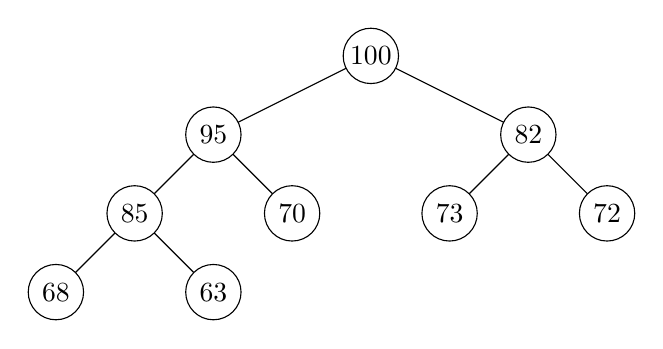
\begin{tikzpicture}
                    \draw (0,5) -- (-2,4) -- (-3,3) -- (-4,2);
                    \draw (-3,3) -- (-2,2);
                    \draw (-2,4) -- (-1,3);
                    \draw (0,5) -- (2,4) -- (3,3);
                    \draw (2,4) -- (1,3);
                    
                    \filldraw[fill=white] (0,5) circle (10pt) node {100};
                    \filldraw[fill=white] (-2,4) circle (10pt) node {95};
                    \filldraw[fill=white] (-3,3) circle (10pt) node {85};
                    \filldraw[fill=white] (-1,3) circle (10pt) node {70};
                    \filldraw[fill=white] (-4,2) circle (10pt) node {68};
                    \filldraw[fill=white] (-2,2) circle (10pt) node {63};
                    
                    \filldraw[fill=white] (2,4) circle (10pt) node {82};
                    \filldraw[fill=white] (3,3) circle (10pt) node {72};
                    \filldraw[fill=white] (1,3) circle (10pt) node {73};
                \end{tikzpicture}
            \end{center}
            \caption{An example Heap}
        \end{figure}
        
        \begin{quote}
            ``A heap container is a binary tree data structure that is not used for searching, [...]
            In a heap data structure the node keys are always larger than their child nodes,
            but their children nodes are not in any particular order. This differs
            from the binary tree, in which the left child is always the smaller node,
            while the right node is always the larger value when compared to their parents.''
            
            \footnotesize
            From Data Structures and Algorithms for Game Developers, by Allen Sherrod, page 328

            \normalsize

            ``Three major characteristics make a heap data structure what it is: (a) A heap is
            a binary tree. (b) A heap is a complete data structure, meaning the rows of nodes are completely
            filled in from left to right without any gaps, [...] (c) Every node in a heap is larger
            than or equal to its child nodes.''

            \footnotesize
            From Data Structures and Algorithms for Game Developers, by Allen Sherrod, page 329            
        \end{quote}

        If a heap has the larger values as parents, it is known as a \textbf{maxheap}.
        Otherwise, if the parents have smaller values than their children, the heap is a \textbf{minheap}.

    \hrulefill

    % -------------------------------------------------------------%
    % - QUESTION --------------------------------------------------%
    % -------------------------------------------------------------%
    \stepcounter{question}
    \begin{question}{\thequestion}{2}

        Identify which of the following are heaps. If a graph is not
        a heap, please specify what makes it invalid.
        
        \begin{center}
            \begin{tikzpicture}draw (0,5) circle (1pt) node[above] {Proto-indo-european};                
            \end{tikzpicture}
        \end{center}

        \begin{enumerate}
            \item[a.] \solution{is a heap}{} \footnote{ From Data Structures and Algorithms for Game Developers, by Allen Sherrod, page 328 }
            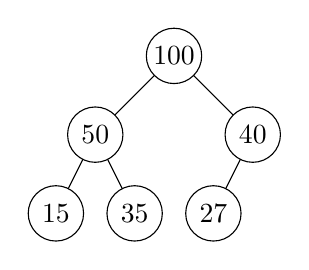
\begin{tikzpicture}
                \draw (0,3) -- (-1,2);
                \draw (0,3) -- (1,2);
                \draw (-1,2) -- (-1.5,1);
                \draw (-1,2) -- (-0.5,1);
                \draw (1,2) -- (0.5,1);
                
                \filldraw[fill=white] (0,3) circle (10pt) node {100};
                \filldraw[fill=white] (-1,2) circle (10pt) node {50};
                \filldraw[fill=white] (1,2) circle (10pt) node {40};
                \filldraw[fill=white] (-1.5,1) circle (10pt) node {15};
                \filldraw[fill=white] (-0.5,1) circle (10pt) node {35};
                \filldraw[fill=white] (0.5,1) circle (10pt) node {27};
            \end{tikzpicture} ~\\~\\

            \item[b.]   \solution{not a heap; it isn't complete.}{} \footnote{ From Data Abstraction \& Problem Solving with C++: Walls and Mirrors 7th ed, by Carrano and Henry, page 489 }
            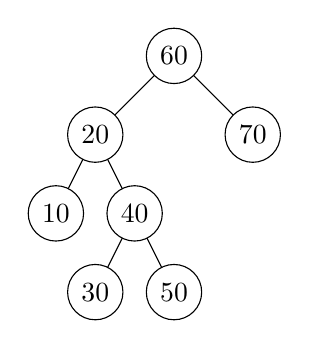
\begin{tikzpicture}
                \draw (0,3) -- (-1,2) -- (-1.5, 1);
                \draw (-1,2) -- (-0.5,1) -- (-1,0);
                \draw (-0.5,1) -- (0,0);
                \draw (0,3) -- (1,2);
                
                \filldraw[fill=white] (0,3) circle (10pt) node {60};
                \filldraw[fill=white] (-1,2) circle (10pt) node {20};
                \filldraw[fill=white] (1,2) circle (10pt) node {70};
                \filldraw[fill=white] (-1.5,1) circle (10pt) node {10};
                \filldraw[fill=white] (-0.5,1) circle (10pt) node {40};
                \filldraw[fill=white] (-1,0) circle (10pt) node {30};
                \filldraw[fill=white] (0,0) circle (10pt) node {50};
            \end{tikzpicture}
        \end{enumerate}

    \end{question}

    \newpage

    \subsection{Implementation}

    Even though heaps are visualized as a binary tree, they are usually
    implemented with an array structure, with the root node (the node with
    the greatest value) being at index 0.

    \begin{figure}[h]
        \begin{center}
            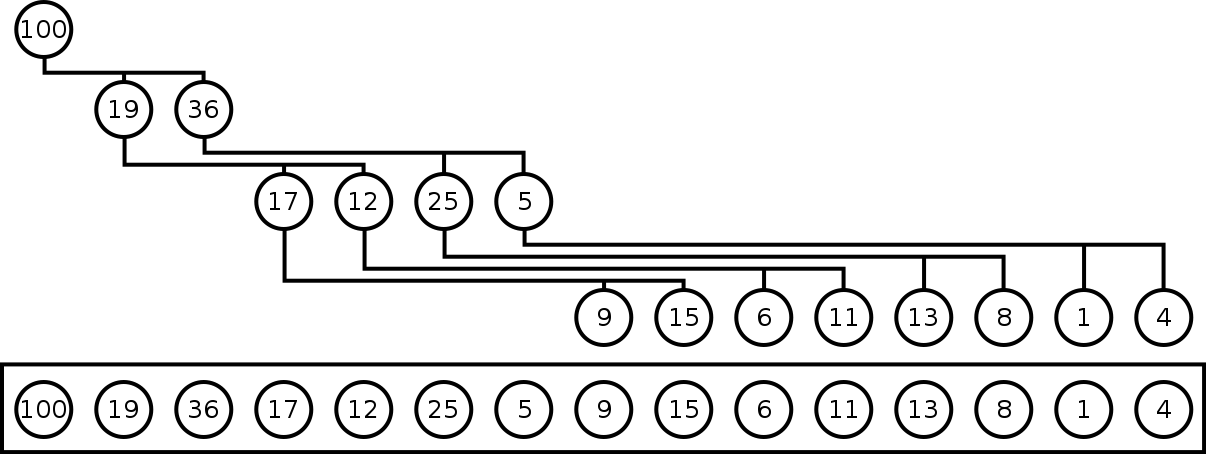
\includegraphics[width=14cm]{images/temp_heap-as-array_wikipedia_maxiantor_cc-share-alike4.png}
        \end{center}

        \caption{``Example of a complete binary max-heap with node keys being integers from 1 to 100 and how it would be stored in an array.'' by Maxiantor;
                    downloaded from https://en.wikipedia.org/wiki/Heap\_data\_structure\#Implementation}
    \end{figure}

    With a heap implemented in this way, you can locate children and parents by modifying the index of a given node at position $i$ (that is, \texttt{item[i]})

    \begin{itemize}
        \item   Its left child, if it exists, is \texttt{items[2 * i + 1]}
        \item   Its right child, if it exists, is \texttt{items[2 * i + 2]}
        \item   Its parent child, if it exists, is \texttt{items[(i - 1) / 2]}
    \end{itemize}
    Remember that only the root in \texttt{items[0]} does not have a parent.
    \footnote{ From Data Abstraction \& Problem Solving with C++: Walls and Mirrors 7th ed, by Carrano and Henry, page 489 }

    \newpage

    % -------------------------------------------------------------%
    % - QUESTION --------------------------------------------------%
    % -------------------------------------------------------------%
    \stepcounter{question}
    \begin{question}{\thequestion}{2}
        Draw the heap that corresponds to the given array.
        % Page 519
        ~\\~\\
        \begin{tabular}{r c}
            & items
            \\ \cline{2-2} 
            0 & \multicolumn{1}{|c|}{Jose}
            \\ \cline{2-2}
            1 & \multicolumn{1}{|c|}{Deepak}
            \\ \cline{2-2}
            2 & \multicolumn{1}{|c|}{Qiang}
            \\ \cline{2-2}
            3 & \multicolumn{1}{|c|}{Anton}
            \\ \cline{2-2}
            4 & \multicolumn{1}{|c|}{Elisa}
            \\ \cline{2-2}
            5 & \multicolumn{1}{|c|}{Mia}
            \\ \cline{2-2}
            6 & \multicolumn{1}{|c|}{}
            \\ \cline{2-2}
            7 & \multicolumn{1}{|c|}{}
            \\ \cline{2-2}
        \end{tabular}
    \end{question} 

    ~\\~\\
    
    \hrulefill

    \subsubsection{Inserting into a heap}

        \begin{quote}
            ``Although a heap is weakly ordered, the purpose of the data structure is
            to allow for fast removal from the top of the heap. When an item is inserted
            into the data structure, it is initially placed on the bottom of the list.
            The element cannot stay at this position because its value might violate the heap condition
            that states that every child must be smaller than its parent. Thus, when an element is inserted
            into the container, it is moved up through the list until it finds an index where the
            element is smaler than its parent but larger than its children.''

            \footnotesize
            From Data Structures and Algorithms for Game Developers, by Allen Sherrod, page 329            
        \end{quote}

        \newpage

        Example: Adding the number 15 to the following heap... ~\\
    
        \begin{tabular}{c c c c}
            Original heap
            &
            Add 15
            &
            Bubble up
            &
            Bubble up

            \\ \\
            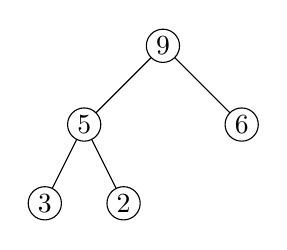
\begin{tikzpicture}
                \draw (0,3) -- (-1,2);
                \draw (0,3) -- (1,2);

                \draw (-1,2) -- (-1.5,1);
                \draw (-1,2) -- (-0.5,1);
                
                \filldraw[fill=white] (0,3) circle (6pt) node {9};
                
                \filldraw[fill=white] (-1,2) circle (6pt) node {5};
                \filldraw[fill=white] (1,2)  circle (6pt) node {6};
                
                \filldraw[fill=white] (-1.5,1)  circle (6pt) node {3};
                \filldraw[fill=white] (-0.5,1)  circle (6pt) node {2};
            \end{tikzpicture}
            &
            
            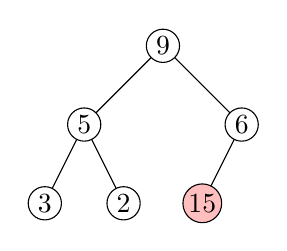
\begin{tikzpicture}
                \draw (0,3) -- (-1,2);
                \draw (0,3) -- (1,2);

                \draw (-1,2) -- (-1.5,1);
                \draw (-1,2) -- (-0.5,1);

                \draw (1,2) -- (0.5,1);
                
                \filldraw[fill=white] (0,3) circle (6pt) node {9};
                
                \filldraw[fill=white] (-1,2) circle (6pt) node {5};
                \filldraw[fill=white] (1,2)  circle (6pt) node {6};
                
                \filldraw[fill=white] (-1.5,1)  circle (6pt) node {3};
                \filldraw[fill=white] (-0.5,1)  circle (6pt) node {2};

                \filldraw[fill=pink] (0.5,1) circle (7pt) node {15};
            \end{tikzpicture}
            &
            
            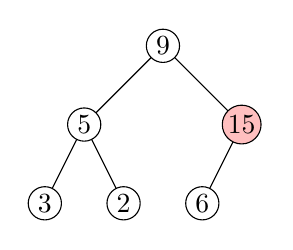
\begin{tikzpicture}
                \draw (0,3) -- (-1,2);
                \draw (0,3) -- (1,2);

                \draw (-1,2) -- (-1.5,1);
                \draw (-1,2) -- (-0.5,1);

                \draw (1,2) -- (0.5,1);
                
                \filldraw[fill=white] (0,3) circle (6pt) node {9};
                
                \filldraw[fill=white] (-1,2) circle (6pt) node {5};
                \filldraw[fill=white] (0.5,1)  circle (6pt) node {6};
                
                \filldraw[fill=white] (-1.5,1)  circle (6pt) node {3};
                \filldraw[fill=white] (-0.5,1)  circle (6pt) node {2};

                \filldraw[fill=pink] (1,2) circle (7pt) node {15};
            \end{tikzpicture}
            &
            
            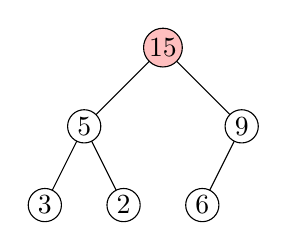
\begin{tikzpicture}
                \draw (0,3) -- (-1,2);
                \draw (0,3) -- (1,2);

                \draw (-1,2) -- (-1.5,1);
                \draw (-1,2) -- (-0.5,1);

                \draw (1,2) -- (0.5,1);
                
                \filldraw[fill=white] (1,2) circle (6pt) node {9};
                
                \filldraw[fill=white] (-1,2) circle (6pt) node {5};
                \filldraw[fill=white] (0.5,1)  circle (6pt) node {6};
                
                \filldraw[fill=white] (-1.5,1)  circle (6pt) node {3};
                \filldraw[fill=white] (-0.5,1)  circle (6pt) node {2};

                \filldraw[fill=pink] (0,3) circle (7pt) node {15};
            \end{tikzpicture}
        \end{tabular}
    \footnote{ From Data Abstraction \& Problem Solving with C++: Walls and Mirrors 7th ed, by Carrano and Henry, page 523 }

    First, the new node is added to the next available space. Again, the Heap fills
    from left to right because it is a complete binary tree.

    If the new location invalidates the heap, then it ``bubbles up'' and it and its parent swap positions.

    It continues bubbling up until (1) its parent is greater than it, and (2) its children are less than it.

    \hrulefill

    % -------------------------------------------------------------%
    % - QUESTION --------------------------------------------------%
    % -------------------------------------------------------------%
    \stepcounter{question}
    \begin{question}{\thequestion}{2}
        With the heap given, draw each step as you insert the new node and
        bubble it up to a valid location. 

        ~\\
        Heap: ~\\~\\
        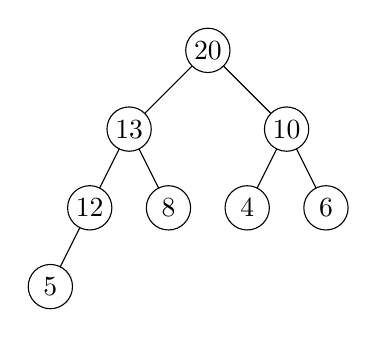
\begin{tikzpicture}
            % From https://www.youtube.com/watch?v=kbkU80mbdcQ
            \draw (-1,3) -- (0,4) -- (1,3);
            \draw (-1.5,2) -- (-1,3) -- (-0.5,2);
            \draw (0.5,2) -- (1,3) -- (1.5,2);
            \draw (-2,1) -- (-1.5,2);
            
            \filldraw[fill=white] (0,4)         circle (8pt) node {20};
            
            \filldraw[fill=white] (-1,3)        circle (8pt) node {13};
            \filldraw[fill=white] (1,3)         circle (8pt) node {10};
            
            \filldraw[fill=white] (-1.5,2)      circle (8pt) node {12};
            \filldraw[fill=white] (-0.5,2)      circle (8pt) node {8};
            
            \filldraw[fill=white] (-2,1)        circle (8pt) node {5};

            \filldraw[fill=white] (0.5,2)       circle (8pt) node {4};
            \filldraw[fill=white] (1.5,2)       circle (8pt) node {6};
        \end{tikzpicture}

        ~\\
        Inserting: 15
    \end{question}

    
    \newpage

    \subsubsection{Removing from a heap}

        \begin{quote}
            ``Removing is done from the top of the heap. When a heap is implemented
            as an array, this means removing element 0 since the element at index 0 is always
            teh root node. Once the root has been removed, the heap is no longer complete
            because of the newly made hole, and it must be replaced with the next elements in line.''
            
            \footnotesize
            From Data Structures and Algorithms for Game Developers, by Allen Sherrod, page 329            
        \end{quote}
		
		% Add more information about a "HeapifyDown" function, or step-by-step how this works.
		NOTE TO SELF: ADD MORE INFO.

        \begin{tabular}{p{4cm} p{4cm} p{4cm}}
            \multicolumn{1}{c}{Heap}
            &
            \multicolumn{1}{c}{Semiheap}
            &
            \multicolumn{1}{c}{Restored heap}

            \\ \\
            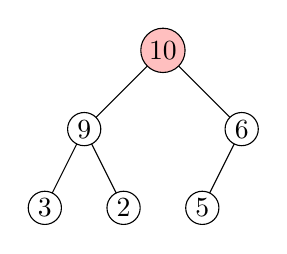
\begin{tikzpicture}
                \draw (0,3) -- (-1,2);
                \draw (0,3) -- (1,2);

                \draw (-1,2) -- (-1.5,1);
                \draw (-1,2) -- (-0.5,1);
                \draw (1,2) -- (0.5,1);
                
                \filldraw[fill=pink] (0,3) circle (8pt) node {10};
                
                \filldraw[fill=white] (-1,2) circle (6pt) node {9};
                \filldraw[fill=white] (1,2)  circle (6pt) node {6};
                
                \filldraw[fill=white] (-1.5,1)  circle (6pt) node {3};
                \filldraw[fill=white] (-0.5,1)  circle (6pt) node {2};
                \filldraw[fill=white] (0.5,1)  circle (6pt) node {5};
            \end{tikzpicture}
            &
            
            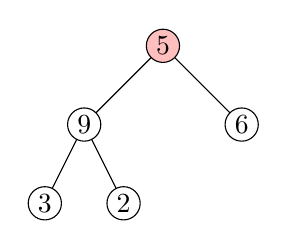
\begin{tikzpicture}
                \draw (0,3) -- (-1,2);
                \draw (0,3) -- (1,2);

                \draw (-1,2) -- (-1.5,1);
                \draw (-1,2) -- (-0.5,1);
                
                \filldraw[fill=pink] (0,3) circle (6pt) node {5};
                
                \filldraw[fill=white] (-1,2) circle (6pt) node {9};
                \filldraw[fill=white] (1,2)  circle (6pt) node {6};
                
                \filldraw[fill=white] (-1.5,1)  circle (6pt) node {3};
                \filldraw[fill=white] (-0.5,1)  circle (6pt) node {2};
            \end{tikzpicture}
            &
            
            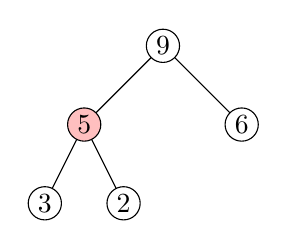
\begin{tikzpicture}
                \draw (0,3) -- (-1,2);
                \draw (0,3) -- (1,2);

                \draw (-1,2) -- (-1.5,1);
                \draw (-1,2) -- (-0.5,1);
                
                \filldraw[fill=white] (0,3) circle (6pt) node {9};
                
                \filldraw[fill=pink] (-1,2) circle (6pt) node {5};
                \filldraw[fill=white] (1,2)  circle (6pt) node {6};
                
                \filldraw[fill=white] (-1.5,1)  circle (6pt) node {3};
                \filldraw[fill=white] (-0.5,1)  circle (6pt) node {2};
            \end{tikzpicture}

            \\
            \multicolumn{1}{c}{\footnotesize Remove 10...}
            &
            \multicolumn{1}{c}{\footnotesize Last entry moved to root}
            &
            \multicolumn{1}{c}{\footnotesize Bubble down}
            \\
            \begin{tabular}{c c c c c c}
                \hline
                \multicolumn{1}{|c|}{\cellcolor{pink}10} &
                \multicolumn{1}{c|}{9} &
                \multicolumn{1}{c|}{6} &
                \multicolumn{1}{c|}{3} &
                \multicolumn{1}{c|}{2} &
                \multicolumn{1}{c|}{5} 
                \\ \hline
                0 & 1 & 2 & 3 & 4 & 5
            \end{tabular}
            &
            \begin{tabular}{c c c c c c}
                \hline
                \multicolumn{1}{|c|}{\cellcolor{pink}5} &
                \multicolumn{1}{c|}{9} &
                \multicolumn{1}{c|}{6} &
                \multicolumn{1}{c|}{3} &
                \multicolumn{1}{c|}{2} &
                \multicolumn{1}{c|}{} 
                \\ \hline
                0 & 1 & 2 & 3 & 4 & 5
            \end{tabular}
            &
            \begin{tabular}{c c c c c c}
                \hline
                \multicolumn{1}{|c|}{9} &
                \multicolumn{1}{c|}{\cellcolor{pink}5} &
                \multicolumn{1}{c|}{6} &
                \multicolumn{1}{c|}{3} &
                \multicolumn{1}{c|}{2} &
                \multicolumn{1}{c|}{} 
                \\ \hline
                0 & 1 & 2 & 3 & 4 & 5
            \end{tabular}
        \end{tabular}

    \footnote{ From Data Abstraction \& Problem Solving with C++: Walls and Mirrors 7th ed, by Carrano and Henry, page 521 }

    When removing an item from a heap, we remove the item at position 0 -- the root.
    In order to maintain the tree structure, we replace that root item with the
    last item in the heap, remembering that the heap fills from left-to-right.

    \newpage

    % -------------------------------------------------------------%
    % - QUESTION --------------------------------------------------%
    % -------------------------------------------------------------%
    \stepcounter{question}
    \begin{question}{\thequestion}{2}
        With the heap given, draw each step as you remove the root,
        replace it with the last node, and then bubble down to
        restore the heap to a valid state. ~\\~\\
        % From https://www.youtube.com/watch?v=ijfPvX2qYOQ

        \begin{center}
            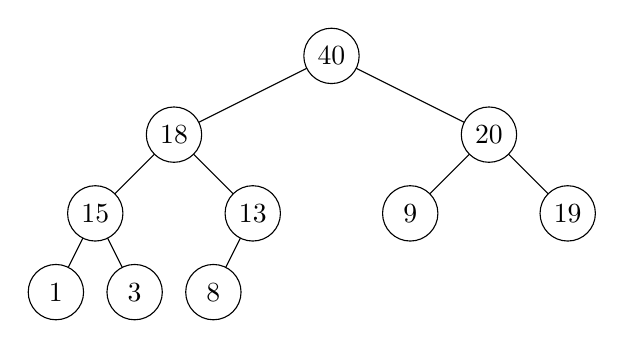
\begin{tikzpicture}
                \draw (-3.5,1) -- (-3,2) -- (-2.5,1);
                \draw (-1.5,1) -- (-1,2);
                \draw (-1,2) -- (-2,3) -- (-3,2);
                \draw (1,2) -- (2,3) -- (3,2);
                \draw (-2,3) -- (0,4) -- (2,3);
                
                \filldraw[fill=white] (0,4)         circle (10pt) node {40};
                
                \filldraw[fill=white] (-2,3)        circle (10pt) node {18};
                \filldraw[fill=white] (-3,2)        circle (10pt) node {15};
                \filldraw[fill=white] (-3.5,1)      circle (10pt) node {1};
                \filldraw[fill=white] (-2.5,1)      circle (10pt) node {3};
                
                \filldraw[fill=white] (-1,2)        circle (10pt) node {13};
                \filldraw[fill=white] (-1.5,1)      circle (10pt) node {8};
                
                \filldraw[fill=white] (2,3)         circle (10pt) node {20};
                \filldraw[fill=white] (1,2)         circle (10pt) node {9};
                \filldraw[fill=white] (3,2)         circle (10pt) node {19};
            \end{tikzpicture}
        \end{center}
    
    \end{question}

\end{document}









